\documentclass[11pt,a4paper]{article}
\usepackage[margin=24mm]{geometry}
\usepackage[utf8]{inputenc}
\usepackage{tikz}
\usetikzlibrary{positioning}
\title{Risk assessment and decision options as SysML-model vocabulary}
\date{Created 2026-10-07 18:12 CEST}
\begin{document}
\maketitle
\paragraph{Scope and estimate.} The halfarm design document holds a NIST SP 800-30 risk register
(15 risks, 5-level likelihood and impact, the I-2 risk-level table, initial and residual values,
mitigating requirements) outside the model. User decision 2026-10-07 18:06: the risk assessment
becomes part of the integrated model, with an Ishikawa (cause--effect) view and decision diagrams
as its views, inside the regular rendering workflow. ETA 4--5 hours. No benchmark.
\paragraph{Semantics.} New file \texttt{data/sysml/meta\_sysml\_risk.hymeko} (imports the structure
vocabulary, which is not modified). Element kinds: \texttt{hazard} (an undesired top outcome, the
head of an Ishikawa diagram), \texttt{risk} (a scenario with initial and residual likelihood and
impact), \texttt{risk\_category} (an Ishikawa bone), \texttt{risk\_cell} (one cell of a
likelihood $\times$ impact table: \texttt{likelihood}, \texttt{impact} $\to$ \texttt{level}),
\texttt{decision}, \texttt{option}; scale \texttt{scale\_level} (consumer levels with
\texttt{rank}). Edges: \texttt{mitigates} (+ requirement\ldots, $-$ risk); \texttt{leads\_to}
(+ risk, $-$ risk $|$ hazard), a cause--effect chain; \texttt{considers} (+ decision, $-$ option\ldots);
option effects \texttt{selects} (+ option, $-$ candidate: replaces the line it is an alternative
of), \texttt{adds} (+ option, $-$ candidate, $\sim$ block it realizes), \texttt{omits}
(+ option, $-$ product), \texttt{overrides} (+ option, $-$ constraint; edge fields \texttt{value},
\texttt{value\_max}, \texttt{basis}), \texttt{introduces} (+ option, $-$ constraint: checked only
in that option). Levels are never stored on a risk: they come from the cells.
\paragraph{Ownership.} Transformation: the vocabulary, a witness
(\texttt{data/sysml/sysml\_risk\_witness.hymeko}) and a compile test; no engine change. Consumer
(\texttt{02\_design/sze/halfarm/model}): the register, cells, hazards, chains, decisions; views
(register and matrix tables, Ishikawa SVG/TikZ, decision DOT) and checks in its \texttt{diagrams/}.
The option evaluator reuses the consumer's requirement checker (scenario = selected set and
constraint values changed, then re-checked).
\paragraph{Tests.} Witness compiles and every kind/edge resolves; the transformation suite stays
green. Consumer: the model reproduces the document register (levels and the summary 2/11/2 initial,
1/12/2 residual); model tests: complete $5\times5$ table, residual $\le$ initial, acceptance rule,
every risk reaches a hazard, a mitigating requirement refuted on the model is reported.
Counter-tests: a removed cell, a residual above initial, a removed \texttt{leads\_to}, a refuted
mitigating requirement, a changed override value each produce exactly the expected finding.
\paragraph{Budget and risks.} 15 risks, 25 cells, a few options: linear. Risk: hazard assignment
and chains are a modelling judgement -- tagged \texttt{<proposed>} for review. Risk: option
assumptions (e.g.\ an enclosure humidity target) are stated on the override edge (\texttt{basis})
and printed with every verdict that depends on them.
\paragraph{State and rollback.} \texttt{feat/material-lobes}, uncommitted changes of 2026-10-06/07;
other workers' files untouched; no git writes from the sandbox. Rollback: delete the two new data
files and the test module; the structure vocabulary is unchanged.
\begin{center}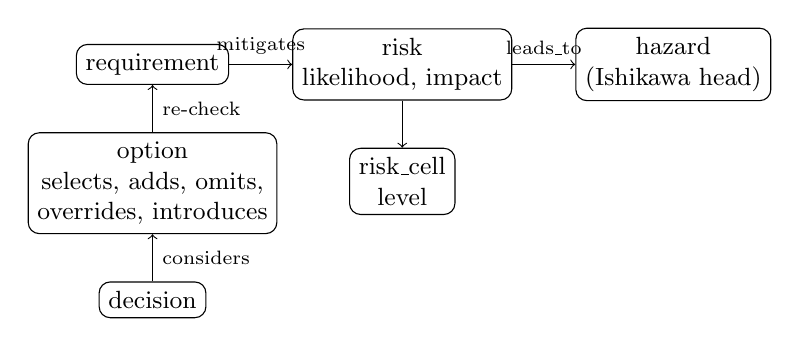
\begin{tikzpicture}[node distance=6mm and 8mm, every node/.style={draw, rounded corners, font=\small, align=center}]
\node (q) {requirement};
\node (r) [right=of q] {risk\\likelihood, impact};
\node (h) [right=of r] {hazard\\(Ishikawa head)};
\node (c) [below=of r] {risk\_cell\\level};
\node (o) [below=of q] {option\\selects, adds, omits,\\overrides, introduces};
\node (d) [below=of o] {decision};
\draw[->] (q) -- node[draw=none, above, font=\scriptsize]{mitigates} (r);
\draw[->] (r) -- node[draw=none, above, font=\scriptsize]{leads\_to} (h);
\draw[->] (r) -- (c);
\draw[->] (d) -- node[draw=none, right, font=\scriptsize]{considers} (o);
\draw[->] (o) -- node[draw=none, right, font=\scriptsize]{re-check} (q);
\end{tikzpicture}
\end{center}
\end{document}
